\section{Modell}

\subsection{Entwurfskonzept}

\begin{figure}[h!]
	\centering
	\def\svgscale{0.75}
	\input{../fig/gph/antenna_concept_1.pdf_tex}
	\caption{Darstellung der separaten idealen Monopol-Antennen.}
	\label{fig:antenna_concept_1}
\end{figure}

Die Entwurf einer einfachen Monopol-Antenne richtet sich nach der dargestellten
Skizze in Abbildung \ref{fig:antenna_concept_1}. Diese zeigt die zwei
\emph{elementaren} Monopolantennen für eine Frequenz von \SI{2.4}{\giga\hertz}
respektive \SI{5.0}{\giga\hertz}. Um nun eine Antenne zu erhalten, welche bei
beiden Frequenzen eine geeginete Abstrahlung zeigt, wurde versucht, diese
beiden \emph{elementaren} Antennen zu kombinieren. Dies ist in der
Abbildung \ref{fig:antenna_concept_2} dargestellt. 

\begin{figure}[h!]
	\centering
	\def\svgscale{0.75}
	\input{../fig/gph/antenna_concept_2.pdf_tex}
	\caption[Darstellung der Zusammenführung der Monopol-Antennen.]{
		Darstellung der Zusammenführung der Monopol-Antennen.
		Die linke Abbildung zeigt die idealisierte Zusammenführung
		der beiden Antennen. Die rechte Abbildung zeigt die
		Prinzipskizze des realisierten Entwurfs im vorgegebenen
		Antennenbereich der Leiterplatte.}
	\label{fig:antenna_concept_2}
\end{figure}

Die Abbildung \ref{fig:antenna_concept_2} zeigt die Prinzipskizze des
realisierten Antennententwurfs. Die Zusammenführung der Antennen erfolgte
empririsch, wobei verschiedene Konzepte untersucht wurden. Der dargestellte
Entwurf zeigt jenes Konzept, welches sich als besonders geeginet erwies.

Die Untersuchung der unterschiedlichen Konzepte zeigte, dass je nach
Entwurf die Antenne eine gute Charakteristik für die eine oder andere
Frequenz zeigte. Hierbei zeigte die Simulation $S_{11}$ Werte von
typischerweise \SI{-30}{\dB}. Da ein empirisches Vorgehen verwendet
wird, wurde für die Auswahl eines passenden Entwurfs ein Vorgehen und
Qualitätskriterium definiert:

\begin{center}
	\emph{
		Wenn der Reflexionskoeffizient $S_{11}$ \\
		nicht für beide Freuenzen $< \SI{-15}{\dB}$ ist, \\
		so ist der Entwurf anzupassen.}
\end{center}

Zunächst wurde ein Konzept verfolgt, bei welchem sich die Antennen
ideal voneinander entfernen, in der Annahme, dass so unerwünschte
Welchselwirkungen der Felder minimal ausfallen. Aufgrund des gemeinsamen
Einspeisepunktes war ein solches Konzept schwierig umzusetzen. Als weiteres
Konzept wurde versucht, die kürzere Antenne aus der Längeren heraus
abzuzweigen.

Die Untersuchungen zeigten jedoch, dass tiefere Werte von $S_{11}$
erreicht werden, wenn die kürzere Antenne nahe an die längere Antenne
geführt wird. Der damit erstellte \emph{ring} schliesst sich dabei
idealerweise bei gleicher Länge beider Pfade.

\begin{figure}[h!]
	\centering
	\footnotesize
	\def\svgscale{0.75}
	\input{../fig/gph/antenna_concept_3.pdf_tex}
	\caption{Darstellung der beobachteten $S_{11}$ Diagramme unterschiedlicher Antennenkonzepte.}
	\label{fig:antenna_concept_1}
\end{figure}


\subsection{Erläuterung zur Modellbildung}
Um zwei Frequenzen bedienen zu können, wurden zwei Antennenteile realisiert, welche sich im Betrieb ergänzen.

\subsubsection{Modell}

\begin{figure}[h!]
	\centering
	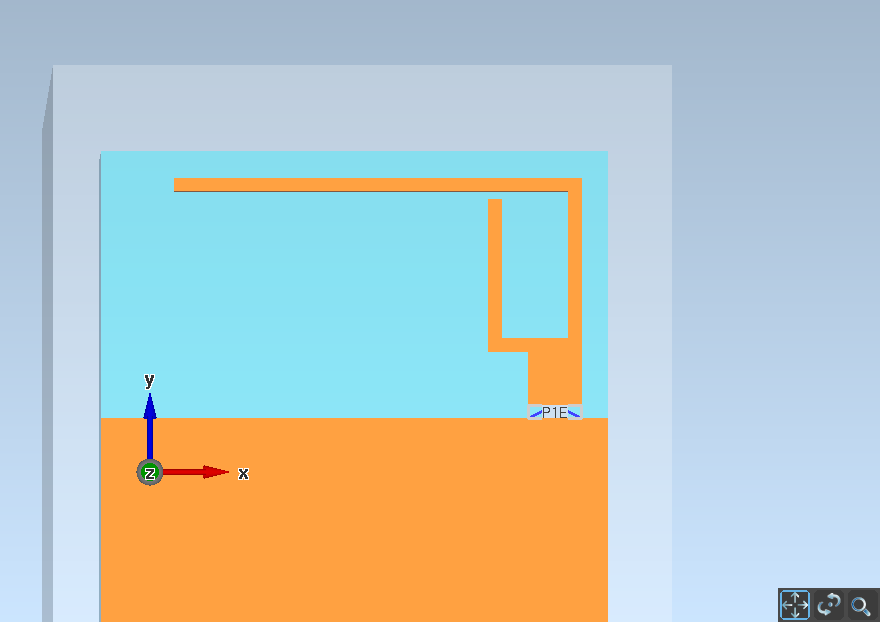
\includegraphics[width=0.7\textwidth]{../fig/plt/crazy_stuff_l4_pcb_v2c_laptop_1a_105_5ghz_3d_pcb_xy.png}
	\caption{2D Modell, Ansicht von oben}
\end{figure}

